\documentclass[paper=a4, fontsize=11pt]{article}

\usepackage{amsmath,amsfonts,amsthm,graphicx} % Math packages
\usepackage[explicit]{titlesec}
\usepackage{fancyhdr} % Custom headers and footers
\usepackage[super]{nth}
\usepackage{parskip}
\usepackage{commath}
\usepackage{amssymb}
\usepackage{mathtools}
\usepackage{enumitem}
\usepackage{textcomp}
\usepackage{wrapfig, framed, caption}
\usepackage{nicefrac}
\usepackage{booktabs,float,siunitx}
\usepackage{subcaption}
\usepackage{bbm}
\usepackage{titling}
\usepackage{multirow}
\usepackage{hyperref}
\usepackage{wrapfig}
\usepackage{forest}
\preauthor{\begin{flushright}\Large}
\postauthor{\par\end{flushright}}

\usepackage{color} %red, green, blue, yellow, cyan, magenta, black, white
\usepackage[margin=0.7in]{geometry}
\usepackage{pdflscape}



%\usepackage [utf8]{inputenc}
%\usepackage[x11names]{xcolor}
%\usepackage[overload]{empheq}
%\colorlet{textcolor}{black}
%\usepackage{listings}
%\usepackage{sectsty} % Allows customizing section commands
%\usepackage{graphicx}
%\usepackage{caption}
%\usepackage{graphicx} 

\newcommand*{\widebox}[2][0.5em]{\fbox{\hspace{#1}$\displaystyle #2$\hspace{#1}}}

\makeatletter
\newcommand*{\centerfloat}{%
  \parindent \z@
  \leftskip \z@ \@plus 1fil \@minus \textwidth
  \rightskip\leftskip
  \parfillskip \z@skip}
\makeatother


%\definecolor{mygreen}{RGB}{28,172,0} % color values Red, Green, Blue
%\definecolor{mylilas}{RGB}{170,55,241}

\def\du#1{\underline{\underline{#1}}}

\pagestyle{fancyplain} % Makes all pages in the document conform to the custom headers and footers
\fancyhead{} % No page header - if you want one, create it in the same way as the footers below
\fancyfoot[L]{} % Empty left footer
\fancyfoot[C]{} % Empty center footer
%\fancyfoot[R]{\thepage} % Page numbering for right footer
\renewcommand{\headrulewidth}{0pt} % Remove header underlines
\renewcommand{\footrulewidth}{0pt} % Remove footer underlines
\setlength{\headheight}{8pt} % Customize the height of the header

%\numberwithin{equation}{section} % Number equations within sections (i.e. 1.1, 1.2, 2.1, 2.2 instead of 1, 2, 3, 4)
%\numberwithin{figure}{section} % Number figures within sections (i.e. 1.1, 1.2, 2.1, 2.2 instead of 1, 2, 3, 4)
%\numberwithin{table}{section} % Number tables within sections (i.e. 1.1, 1.2, 2.1, 2.2 instead of 1, 2, 3, 4)

\setlength\parindent{0pt} % Removes all indentation from paragraphs - comment this line for an assignment with lots of text

%\titleformat{\section}{\normalfont\Large\bfseries}{}{0em}{#1}


%\renewcommand\thesubsection{\alph{subsection}}


%----------------------------------------------------------------------------------------
%	TITLE SECTION
%----------------------------------------------------------------------------------------

\newcommand{\horrule}[1]{\rule{\linewidth}{#1}} % Create horizontal rule command with 1 argument of height

\newcommand{\mychar}[1]{%
  \begingroup\normalfont
  \includegraphics[height=0.8em]{#1}%
  \endgroup
}

%\newcommand{\abs}[1]{\left\lvert#1\right\rvert}

\definecolor{fblue}{RGB}{92,144,192}
\definecolor{fgreen}{RGB}{34,162,70}

\newcommand\myfolder[2][fblue]{%
\begin{tikzpicture}[overlay]
\begin{scope}[xshift=20pt]
\filldraw[rounded corners=1pt,fill=#1,draw=white,double=black]
  (-23pt,10pt) -- ++(3pt,5pt) -- ++(18pt,0pt) -- ++(40:3pt) -- ++(9pt,0pt) -- ++(-40:3pt)
  -- (20pt,15pt) -- (23pt,10pt) -- cycle;
\filldraw[rounded corners,draw=white,double=black,top color=#1,bottom color=#1!30]
  (-22pt,-12pt) -- ++(44pt,0pt) -- (25pt,12pt) coordinate (topr) -- ++(-50pt,0pt) coordinate (topl) -- cycle;
\end{scope}  
\end{tikzpicture}%
\makebox[40pt]{\raisebox{-3pt}{{\footnotesize\ttfamily#2}}}%
}
\newcommand\myfile[2][fblue]{%
{\footnotesize\ttfamily#2}%
}

\newcommand*\circled[1]{\tikz[baseline=(char.base)]{
            \node[shape=circle,draw,inner sep=0.4pt] (char) {#1};}}

\title{	
\normalfont \normalsize \vspace{-1cm}
\textsc{ECE4053: Power System Analysis} \\ [14pt]
\horrule{0.5pt} \\[0.1cm]
\huge Lab 1 - Intro to PSS/E \\
\horrule{2pt} \\[0.2cm]
}
\author{}
\date{}

\begin{document}

\maketitle

%----------------------------------------------------------------------------------------
%	QUESTION 1
%----------------------------------------------------------------------------------------
\vspace{-1.5cm}
\section{Welcome!}
For the first lab of ECE4053 we will introduce a software called Power System Simulator for Engineering (PSS/E). This software is widely used in industry and will also be used in our future labs. We will start from novice level, but by the end of this unit you will be experts in using PSS/E. Let's begin!

\section{Types of simulation software}
In the lectures we have learnt the theory to manually analyse a power system; in industry engineers typically use computer software that automate this theory. There are two main types of simulations: Root Mean Square (RMS) and Electromagnetic Transient (EMT). 

Software, like PSS/E, that perform RMS simulations are suitable for modelling an entire grid and works by calculating the RMS value of the phasor corresponding to the fundamental frequency. Meanwhile, software performing EMT simulations calculate the instantaneous values for voltage and current. The computational effort required for EMT simulations mean they are typically not used on a grid wide scale.

Hopefully we will look into EMT simulations at the end of this unit but if you are interested you can looking into software such as PSCAD or PowerFactory. \textbf{Question:} can you name an advantage of EMT simulation over RMS simulation and vice versa?

\section{Installing PSS/E}
This semester all labs will be conducted remotely. Therefore, it is essential that you are able to run PSS/E on your computer (if you do not have access to a computer please let the demonstrater know). There are two options - please choose whichever is most convenient for you.

\subsection{Local installation of PSS/E Xplore 34}
PSS/E Xplore 34 is a free version of PSS/E distributed by Siemens. Compared with the full version, PSS/E Xplore 34 is limited to only work with 50 buses but this will be sufficient for the labs for this unit. To install PSS/E Xplore 34, please complete the form \href{https://new.siemens.com/global/en/products/energy/services/transmission-distribution-smart-grid/consulting-and-planning/pss-software/psse-xplore-order-form.html}{here}. Alternatively, you can download \texttt{PSSEXplore340302.exe} from the Moodle webpage. Please note that PSS/E is designed for Microsoft Windows.
\smallbreak
\textbf{Pro:} can work offline; \textbf{Con:} requires Microsoft Windows operating system

\subsection{MoVE version of PSS/E 34}
The full license of PSS/E 34 has been ported onto MoVE, which can be accessed \href{https://move.monash.edu/Citrix/MoveStoreWeb/}{here}. Please log into okta with your Monash credentials. If it is your first time using MoVE you will be prompted to install the Citrix Receiver, please follow the onscreen directions. Once you have logged into MoVE, click the search field and type ``PSSE''. The app called Siemens PTI PSSE should appear, please click on this to open PSS/E. You will have to give Citrix permission to read/write to your hard disk.
\smallbreak
\textbf{Pro:} operating system independent; \textbf{Con:} requires constant Internet connection

\section{PSS/E filetypes}
Please download \texttt{Lab1\_files.zip} from Moodle and extract the contents onto your hard drive. You should have the following file structure:

\begin{figure} [h]
\centering
\begin{forest}
	for tree={
		font=\sffamily,
		grow'=0,
		inner ysep=12pt,
		child anchor=west,
		parent anchor=south,
		anchor=west,
		calign=first,
		edge=densely dotted,
		edge path={
			\noexpand\path [draw, \forestoption{edge}]
			(!u.south west) +(12.5pt,0) |- (.child anchor)\forestoption{edge label};
		},
		before typesetting nodes={if n=1 {insert before={[,phantom,minimum height=18pt]}} {}},
		fit=band,
		before computing xy={l=25pt},
		for children={s sep-=0.8em}
	}
[{\myfolder[fgreen]{Lab1\_files}}
  [{\myfolder{taskA}}
    [{\myfile{IEEE14bus.sav}}]
    [{\myfile{IEEE14bus.sld}}]
    [{\myfile{readme.txt}}]
  ]
  [{\myfolder{taskB}}
    [{\myfile{taskB.raw}}]
  ]
]
\end{forest}
\end{figure}

Since it is our first time using PSS/E we will explain the types of files you will encounter when using PSS/E. The first file type we will encounter are \texttt{.sav} files, referred to as ``saved cases''. A saved case contains all the data that PSS/E needs to construct a model of the power system. The saved case also stores analysis results from previous simulation.

The next new type of file we will encounter are \texttt{.sld} files, referred to as ``single line diagrams''. A single line diagram is a visual way of representing a power system that you may be familiar from the lectures and tutorials. There are symbols to represent buses, branches, loads, generators, transformers, etc. and PSS/E allows us to customise these to our requirements.

In Task A of this lab, we will explore an example saved case and single line diagram. Then in Task B, we will learn how to create a saved case and single line diagram for a simple power system.

\section{Task A}
\subsection{The Graphical User Interface (GUI)}
When we open PSS/E we are greeted by the GUI. In Fig. \ref{fig:1} below the key areas of the GUI are highlighted.

\subsubsection*{Activities}
\begin{enumerate}
\item[\textbf{5.1.1}] In Table \ref{table:1} there is are brief descriptions of the functions of these key areas. Can you fill out the last column of Table \ref{table:1} by referring to Fig \ref{fig:1}?
\item[\textbf{5.1.2}] Imagine you accidentally closed the output bar. How can you get it? (Hint: Click \textbf{\textcolor{gray}{View}} on the menu bar.) 
\end{enumerate}

\begin{figure}[h]
\centering
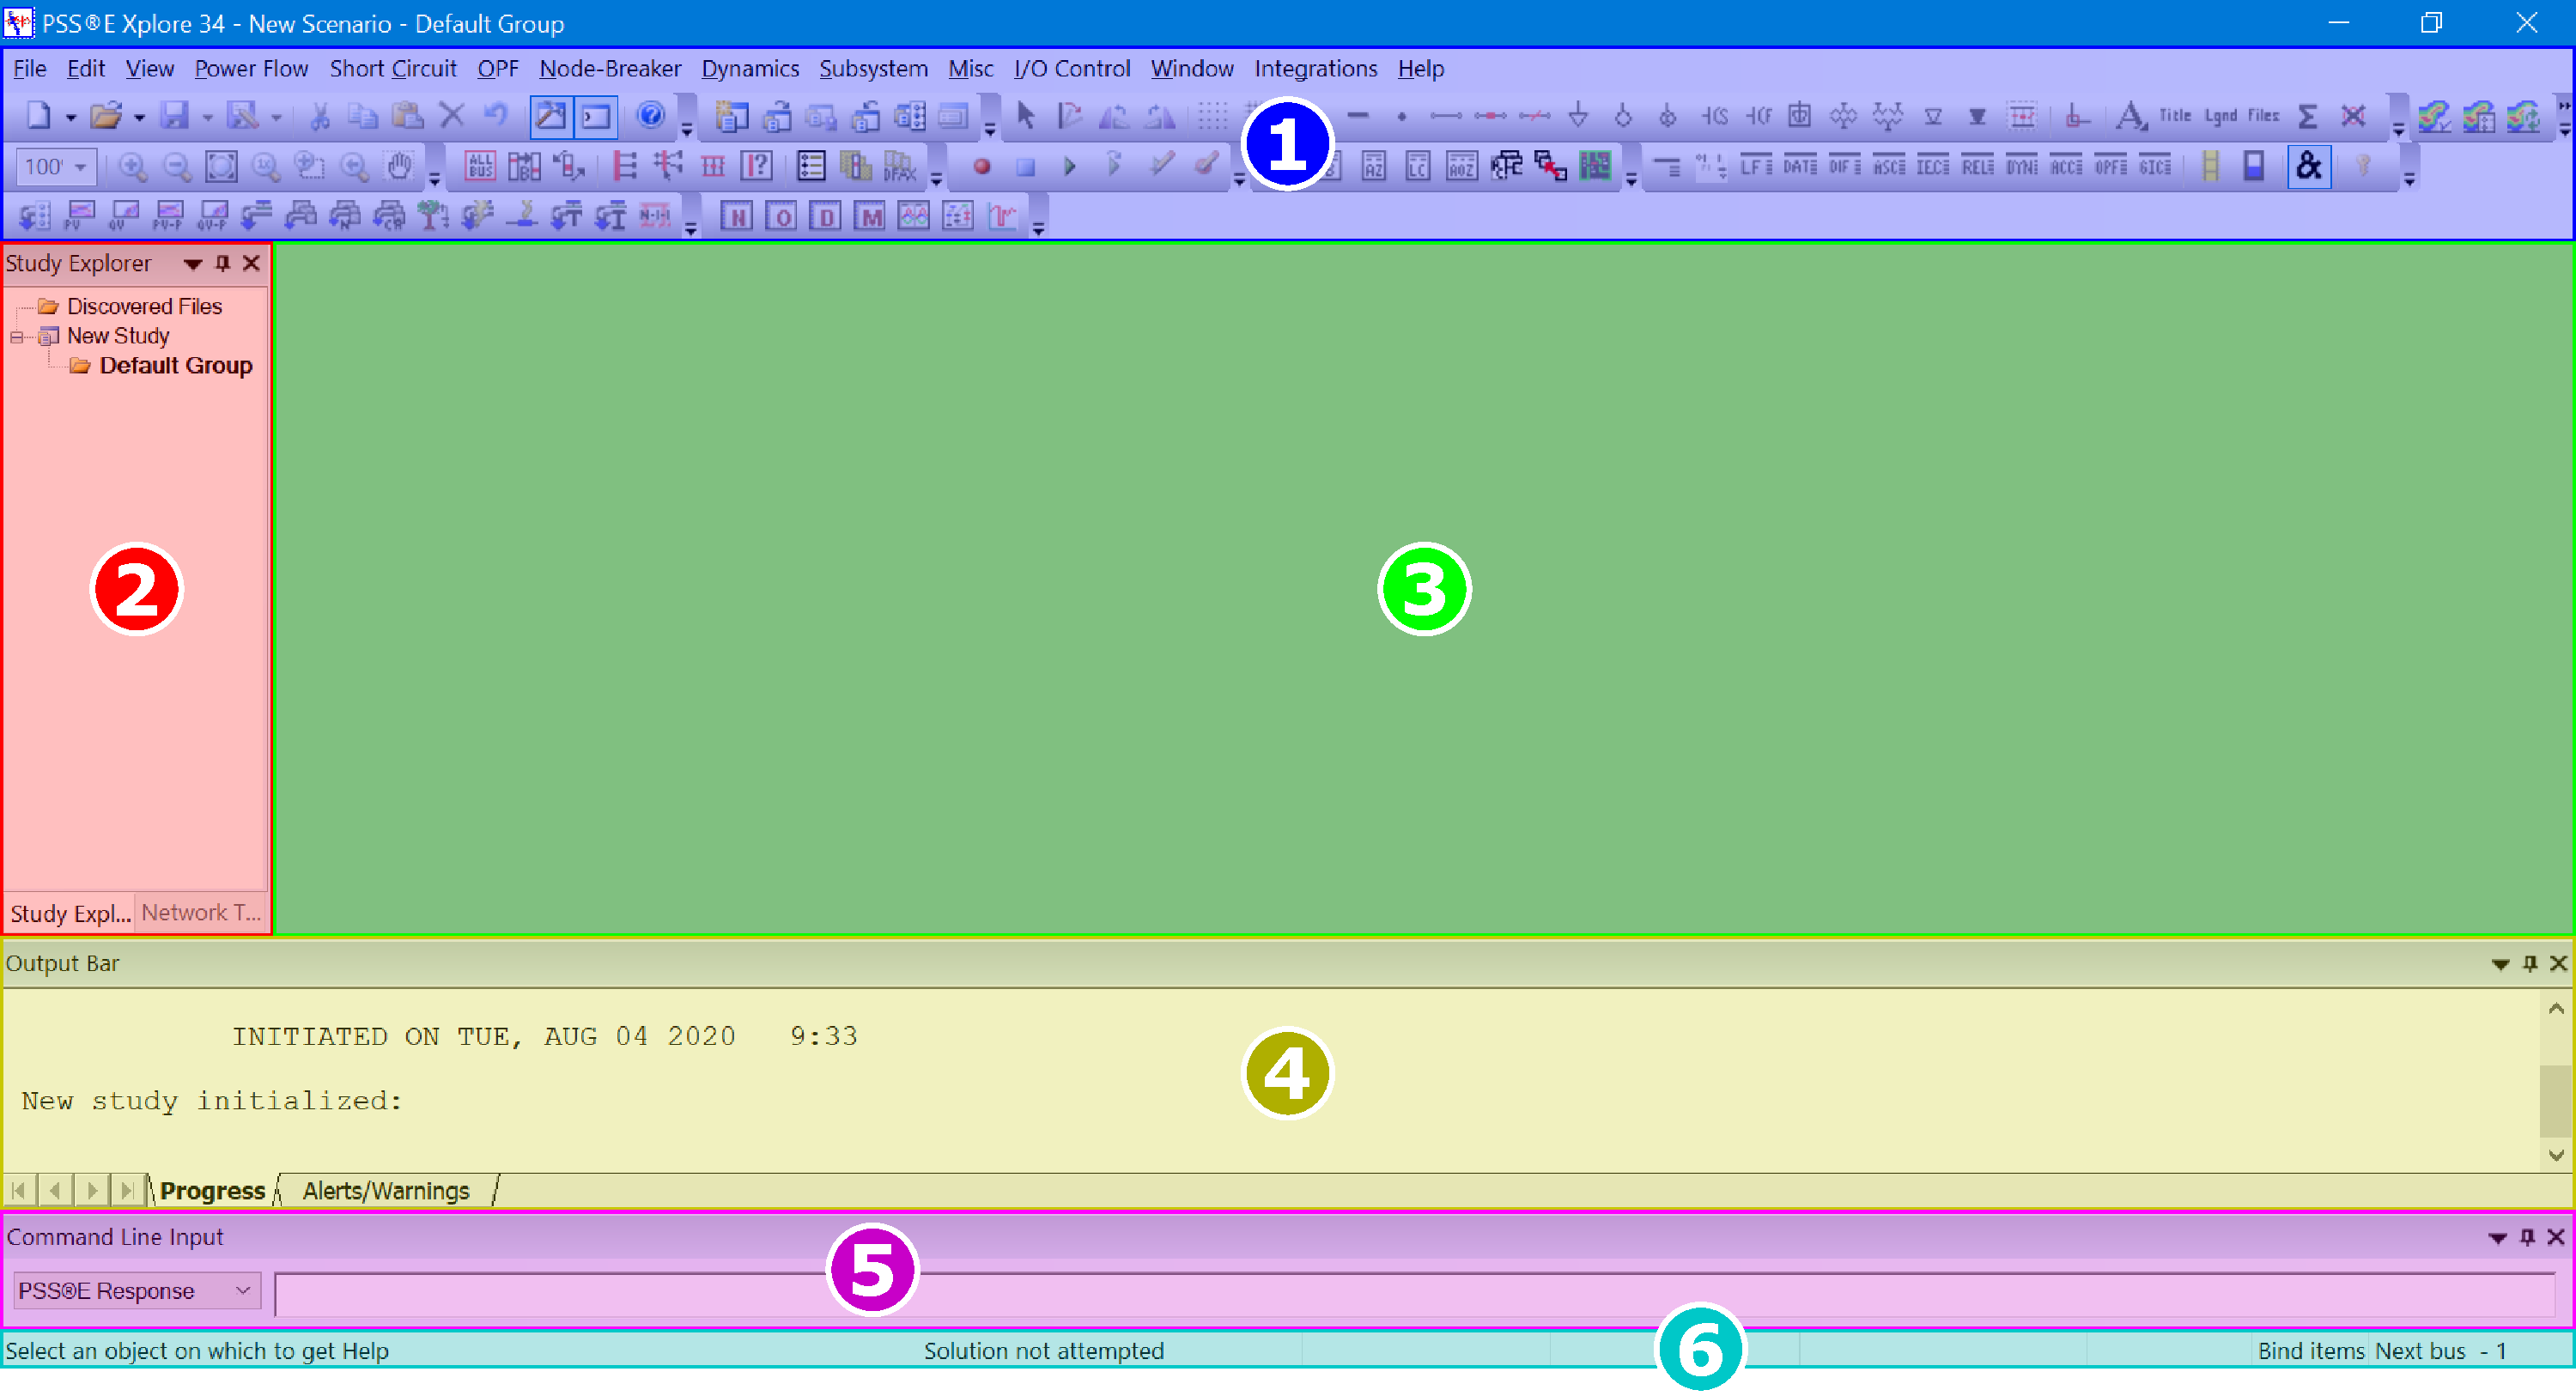
\includegraphics[scale=0.32]{fig1_gui.pdf}
\caption{Key areas of the GUI}
\label{fig:1}
\end{figure}

\begin{table}[h]
\caption{Description of areas of GUI}
\centering
\begin{tabular}{|l|l|l|}
\hline &&\\[-1em]
\textbf{Name}			& \textbf{Functions}                                     				& \textbf{Reference to Fig. 1}			\\ \hline &&\\[-1em]
Main Area				& Spreadsheets, single line diagrams, plots              			& \multicolumn{1}{c|}{\circled{3}}		\\ \hline &&\\[-1em]
Output Bar				& Progress messages, alerts, warnings, report outputs			& 										\\ \hline &&\\[-1em]
Status bar				& Provides explanatory text, status of project         				& 										\\ \hline &&\\[-1em]
Menu and Toolbars		& Open files, run activities                             					& 										\\ \hline &&\\[-1em]
Command Line Input	& Submit commands to PSS/E engine, use Python intepreter		&										\\ \hline &&\\[-1em]
Study Explorer			& Tree views, navigation                                 				& 										\\ \hline 
\end{tabular}
\label{table:1}
\end{table}

\subsection{Check the default settings}
Every time you open PSS/E, it is a good idea to check the program settings. Click \textbf{\textcolor{gray}{Misc \textgreater \phantom{ }Change program settings (OPTN)...}} on the menu bar to open up a dialogue box. 
\begin{figure}[h]
\centering
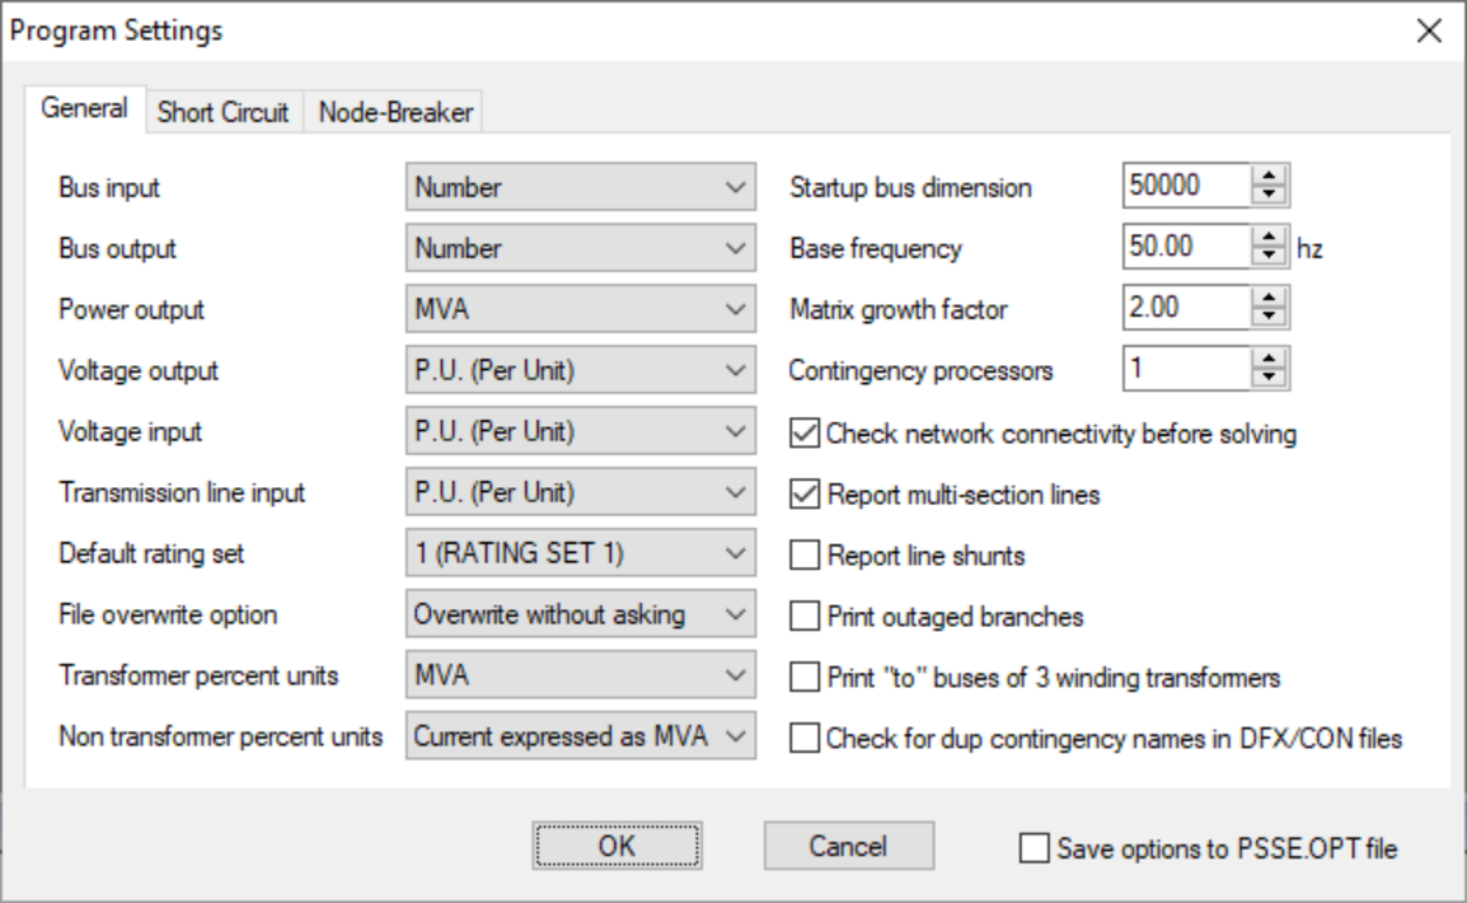
\includegraphics[scale=0.32]{fig2_settings.pdf}
\caption{Key areas of the GUI}
\label{fig:2}
\end{figure}

Check the settings in the ``General'' tab matches Fig. \ref{fig:2} and click the \textbf{\textcolor{gray}{OK}} button. Note if you are using PSS/E Xplore 34, the ``Startup bus dimension'' field will be greyed out -- this will not be an issue for our labs.


\subsection{Opening a saved case}
To open a file use the menu bar: \textbf{\textcolor{gray}{File \textgreater \phantom{ }Open \textgreater \phantom{ }File}}. Alternatively click the \mychar{open.png} icon on the toolbar. Navigate to your local hard drive where you extracted \texttt{Lab1\_files} in Section 4. Now go into the \texttt{taskA} folder and select \texttt{IEEE14bus.sav}. Verify your screen looks like Fig. \ref{fig:3} and click the \textbf{\textcolor{gray}{Open}} button.

\begin{figure}[h]
\centering
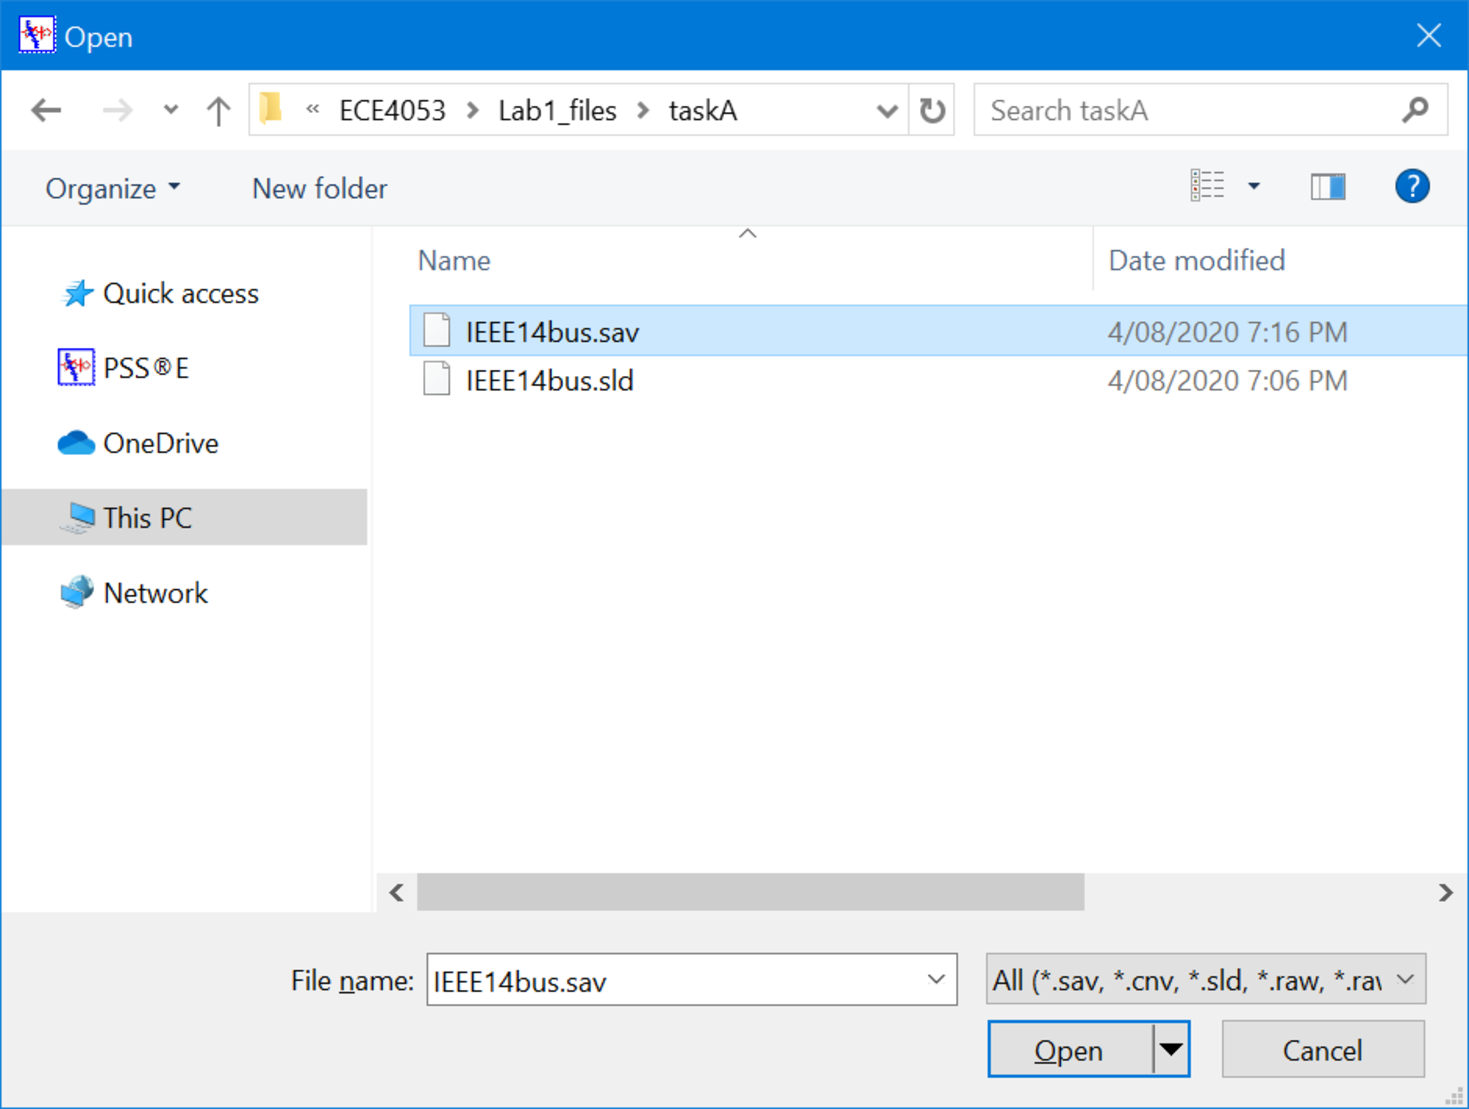
\includegraphics[scale=0.32]{fig3_opensav.pdf}
\caption{Opening a saved case}
\label{fig:3}
\end{figure}

\newpage
\subsection{Using the spreadsheet viewer}
Upon opening the saved case a spreadsheet viewer should appear in the main area as shown in Fig. \ref{fig:4}. 

\begin{figure}[h]
\centering
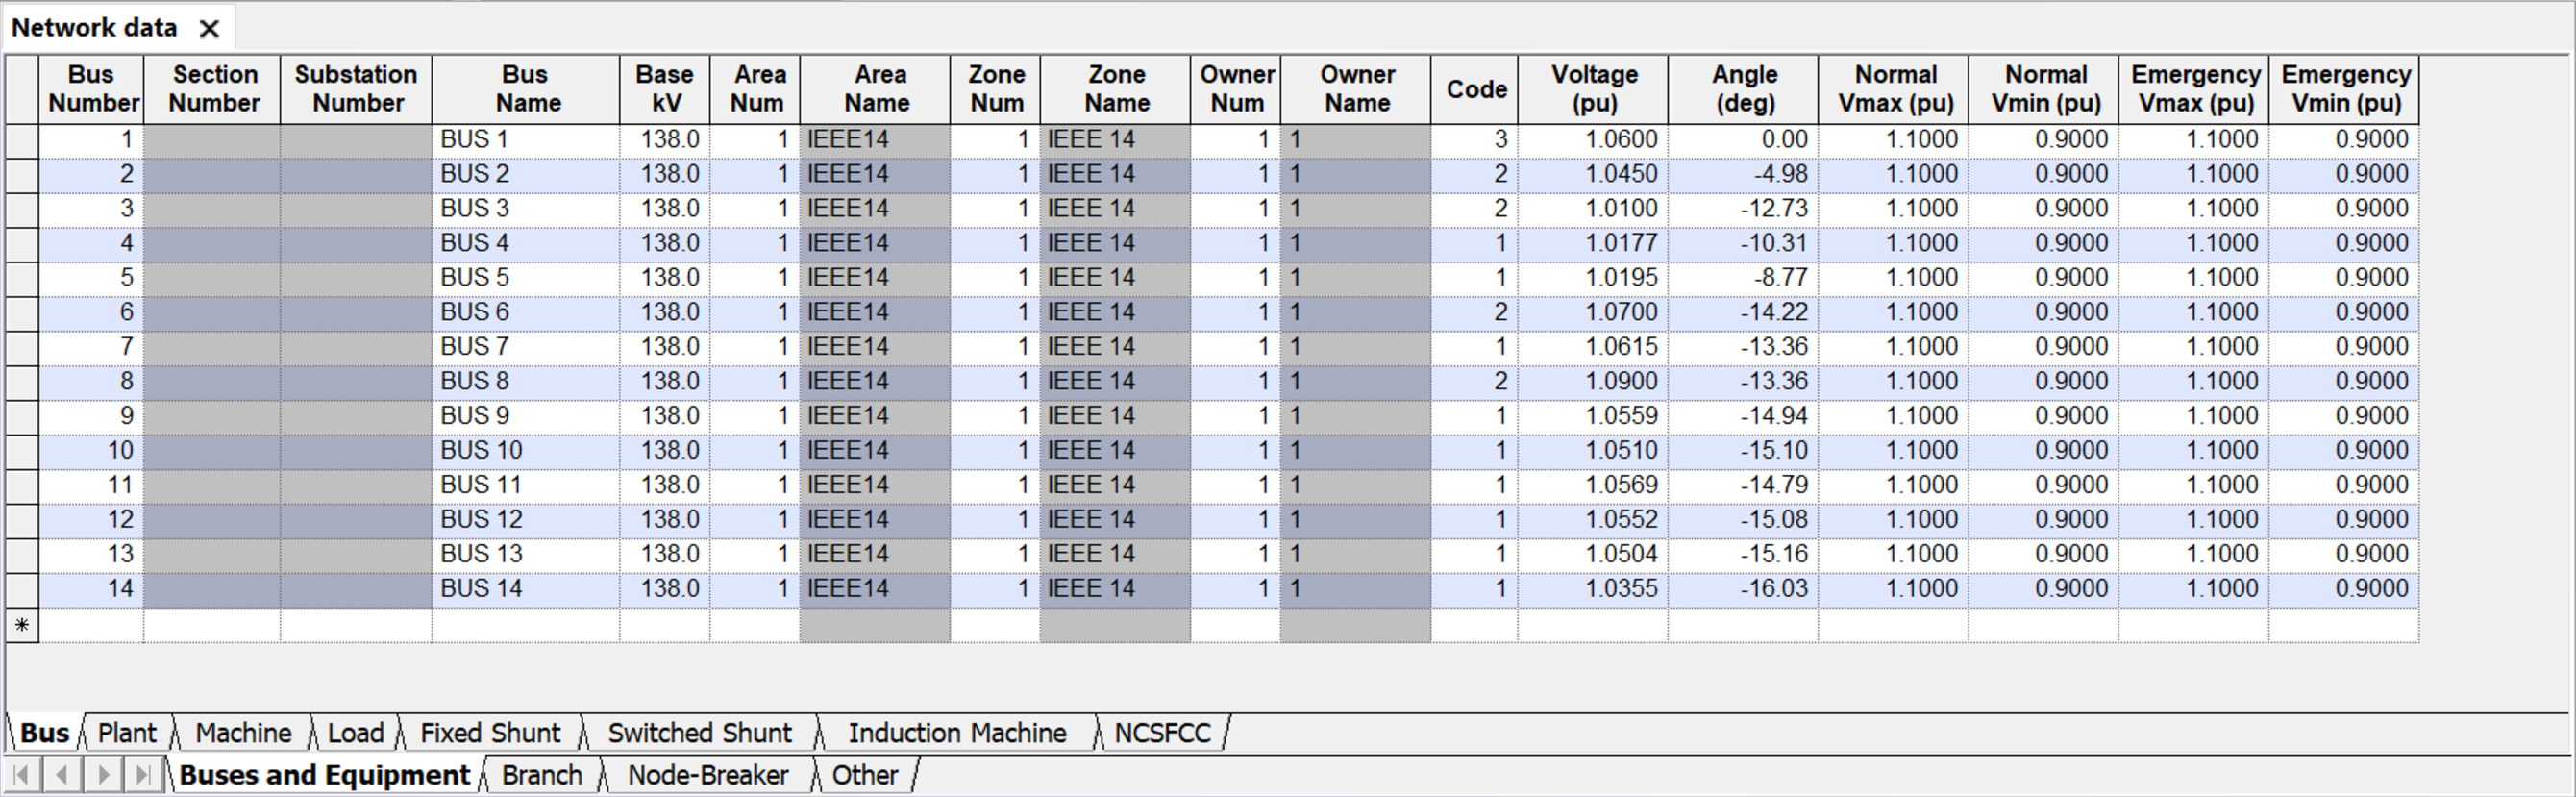
\includegraphics[scale=0.32]{fig4_spreadsheet.pdf}
\caption{Spreadsheet viewer}
\label{fig:4}
\end{figure}

To navigate to different spreadsheets there are a set of tabs at the bottom. These spreadsheets contain the full set of information about the power system model so it is important for us to become familiar with finding relevant information. 

\subsubsection*{Activities}
\begin{enumerate}
\item[\textbf{5.4.1}] How many buses does this power system contain? Which bus is the swing bus and what is its purpose?
\item[\textbf{5.4.2}] How many generators does this power system contain? What is the largest generating unit?
\item[\textbf{5.4.3}] Which bus contains the load that uses the most active power?
\item[\textbf{5.4.4}] Are there any shunt elements?
\item[\textbf{5.4.5}] How many transformers are in this power system?
\item[\textbf{5.4.6}] On Fig. \ref{fig:5} the buses, generators and loads have been drawn. Can you complete the single line diagram by connecting the appropriate buses? (Hint: look at the Branches spreadsheet)
\end{enumerate}

\begin{figure}[t]
\centering
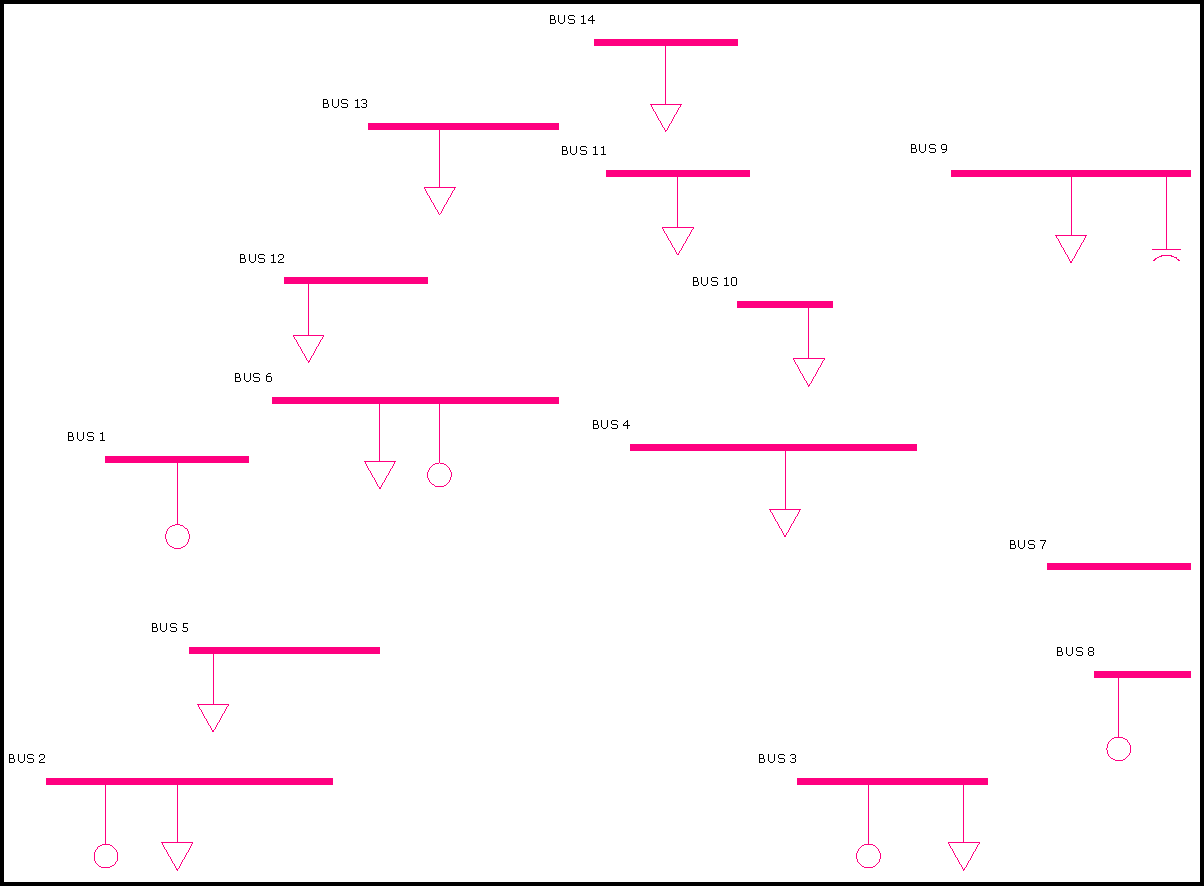
\includegraphics[width=\linewidth]{fig5_diagram.pdf}
\caption{Task A power system}
\label{fig:5}
\end{figure}

\newpage
\subsection{Opening up a diagram}
From Activity 5.4.6 it should be clear that although the spreadsheet contains all the data about the power system in tabular form, it still requires some work to produce a single line diagram. Luckily, PSS/E also has a feature to produce diagrams so that we can visually interact with the power system. To open a diagram use the menu bar: \textbf{\textcolor{gray}{File \textgreater \phantom{ }Open \textgreater \phantom{ }File}}. Alternatively click the \mychar{open.png} icon on the toolbar. Navigate to your local hard drive where you extracted \texttt{Lab1\_files} in Section 4. Now go into the \texttt{taskA} folder and select \texttt{IEEE14bus.sld} and click the \textbf{\textcolor{gray}{Open}} button.

Now we observe that a diagram viewer opens in the main area as shown in Fig. \ref{fig:6} (NB: to go back to the spreadsheet viewer simply use the ``Network data'' tab at the top of the main area). To navigate the diagram there is are a set of useful icons on the second row of the tool bar: \mychar{zoom.png}

\subsubsection*{Activities}
\begin{enumerate}
\item[\textbf{5.5.1}] Use the menu bar \textbf{\textcolor{gray}{Diagram \textgreater \phantom{ }Statistics}} to verify your answers to activity 5.4.1-5.4.5.
\item[\textbf{5.5.2}] Use the ``Zoom extent'' icon to fit the diagram on the page. Now verify your answer to activity 5.4.6.
\item[\textbf{5.5.3}] Use the menu bar \textbf{\textcolor{gray}{Diagram \textgreater \phantom{ }Show Animated Flows}} to view an animation.
\end{enumerate}

\begin{figure}[t]
\centering
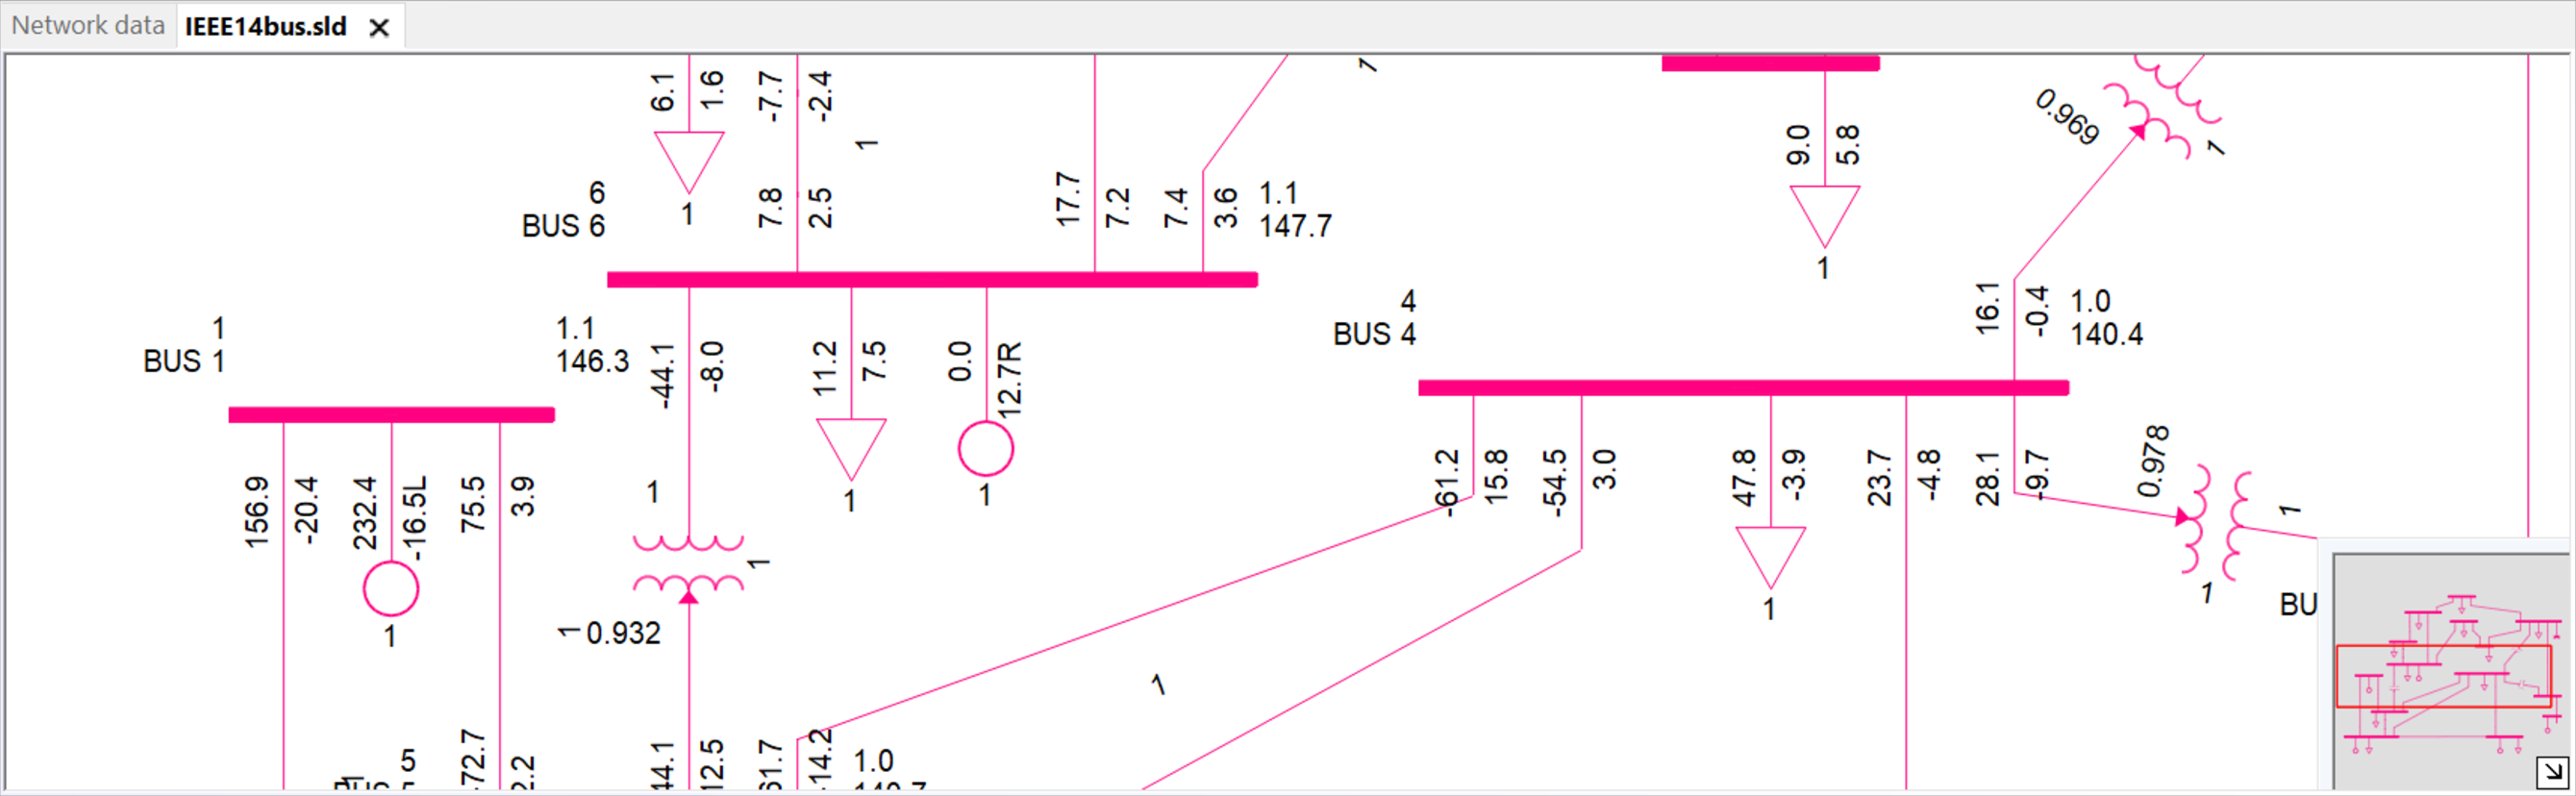
\includegraphics[scale=0.32]{fig6_sldviewer.pdf}
\caption{Single line diagram viewer}
\label{fig:6}
\end{figure}

\newpage
\section{Task B}

\subsection{A toy power system}
For this task we are going to investigate how to create a saved case from raw data and then how to produce a diagram. Fig. \ref{fig:7} depicts the power system we will enter into PSS/E. Please study it carefully since we will be using this toy power system in our future labs. Below is paragraph to help interpret the diagram and set some context:

\begin{quote}
A substation ``Metro'' in a metropolitan area in a remote mining area supplies the town load by 132/33kV transformers and loads at 132kV for the mine at the town, ``Mine A'' and a plant for processing of minerals, ``MinProc''. ``Metro'' is supplied at 132kV by a 30 km double circuit line from the gas power station ``Gas'' and by a 100km double circuit 132 kV line from a hydro power station ``Hydro''. ``Mine A'' has a continuous load of 50MW, MinProc has a continuous load of 100MW and the Town has a maximum load of 95MW. The gas power station has three generating units of 55MW. The hydro power station has three generating units of 65MW. The gas station operates on full rated power and the hydro power station meets the balance of load and generation. Another mine ``Mine B'' is supplied by a 150km single circuit line from the hydro power station and a 80 km 132kV line from the metropolitan substation. Mine B has a load of 50MW.
\end{quote}

\bigbreak

\begin{figure}[h]
\centering
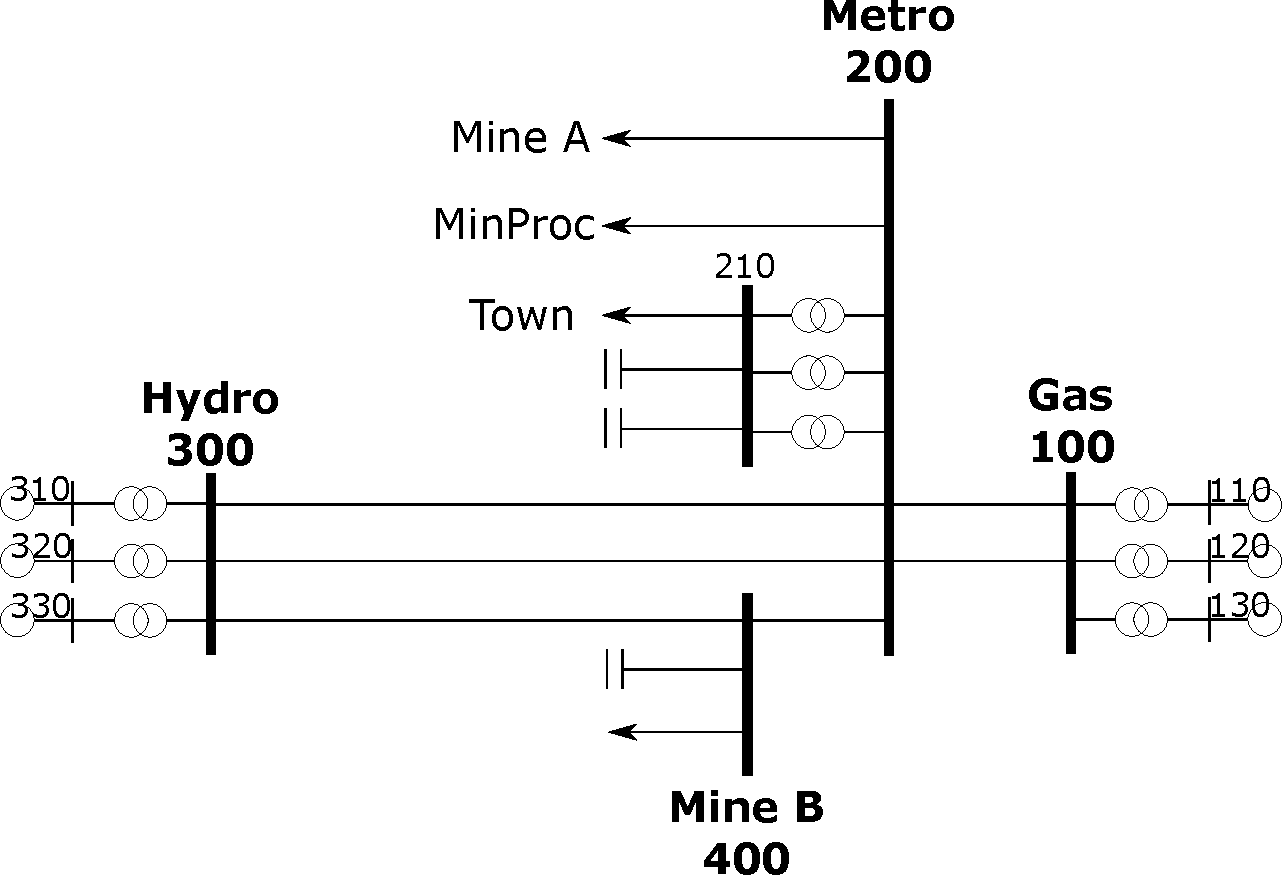
\includegraphics[width=0.8\linewidth]{fig7_taskb.pdf}
\caption{A toy power system}
\label{fig:7}
\end{figure}

\subsection{Tabular data}
To fully define the model of the power system we are provided with seven tables: bus data, branch data, load data, shunt data, generator voltage data, generator machine data and transformer data. These tables are provided below:

\begin{table}[h]
\caption{Bus Data}
\centering
\begin{tabular}{|c|c|c|c|}
\hline &&&\\[-1em]
\textbf{Bus No.} & \textbf{Bus Name} & \textbf{Base Voltage (kV)} & \textbf{Type} \\ \hline &&&\\[-1em]
100              & Gas\_132          & 132                        & PQ            \\ \hline &&&\\[-1em]
110              & Gas1\_mc          & 18                         & PV            \\ \hline &&&\\[-1em]
120              & Gas2\_mc          & 18                         & PV            \\ \hline &&&\\[-1em]
130              & Gas3\_mc          & 18                         & PV            \\ \hline &&&\\[-1em]
200              & Metro132          & 132                        & PQ            \\ \hline &&&\\[-1em]
210              & Metro33           & 33                         & PQ            \\ \hline &&&\\[-1em]
300              & Hydro132          & 132                        & PQ            \\ \hline &&&\\[-1em]
310              & Hyd1\_Mc          & 16                         & SLACK         \\ \hline &&&\\[-1em]
320              & Hyd2\_Mc          & 16                         & PV            \\ \hline &&&\\[-1em]
330              & Hyd3\_Mc          & 16                         & PV            \\ \hline &&&\\[-1em]
400              & MineB             & 132                        & PQ            \\ \hline
\end{tabular}
\label{table:2}
\end{table}

\begin{table}[h]
\caption{Branch Data}
\centering
\begin{tabular}{|c|c|c|c|c|c|c|}
\hline &&&&&&\\[-1em]
\textbf{From Bus No.} & \textbf{To Bus No.} & \textbf{ID} & \textbf{Line R (pu)} & \textbf{Line X (pu)} & \textbf{Charging B (pu)} & \textbf{Rate1 (I as MVA)} \\ \hline &&&&&&\\[-1em]
100                   & 200                 & 1           & 0.006                & 0.045                & 0.022                    & 120                       \\ \hline &&&&&&\\[-1em]
100                   & 200                 & 2           & 0.006                & 0.045                & 0.022                    & 120                       \\ \hline &&&&&&\\[-1em]
200                   & 300                 & 1           & 0.02                 & 0.15                 & 0.07                     & 120                       \\ \hline &&&&&&\\[-1em]
200                   & 300                 & 2           & 0.025                & 0.20                 & 0.09                     & 120                       \\ \hline &&&&&&\\[-1em]
200                   & 400                 & 1           & 0.016                & 0.12                 & 0.055                    & 120                       \\ \hline &&&&&&\\[-1em]
300                   & 400                 & 1           & 0.035                & 0.22                 & 0.10                     & 140                       \\ \hline
\end{tabular}
\label{table:3}
\end{table}


\begin{table}[!htb]
	\begin{minipage}{.4\linewidth}
		\caption{Load Data}
		\centering
		\begin{tabular}{|c|c|c|c|}
		\hline &&&\\[-1em]
		\textbf{Bus No.} & \textbf{ID} & \textbf{P (MW)} & \textbf{Q (Mvar)} \\ \hline &&&\\[-1em]
		200              & 1           & 50              & 16                \\ \hline &&&\\[-1em]
		200              & 2           & 100             & 29                \\ \hline &&&\\[-1em]
		210              & 1           & 95              & 33                \\ \hline &&&\\[-1em]
		400              & 1           & 50              & 18                \\ \hline
		\end{tabular}
	\end{minipage}%
	\begin{minipage}{.3\linewidth}
		\caption{Capacitor Data}
		\centering
		\begin{tabular}{|c|c|c|}
		\hline &&\\[-1em]
		\textbf{Bus No.} & \textbf{ID} & \textbf{B (Mvar)} \\ \hline &&\\[-1em]
		210              & 1           & 12               \\ \hline &&\\[-1em]
		210              & 2           & 15               \\ \hline &&\\[-1em]
		400              & 1           & 10               \\ \hline
		\end{tabular}
	\end{minipage}%
	\begin{minipage}{.3\linewidth}
		\caption{Generator Voltage Data}
		\centering
		\begin{tabular}{|c|c|}
		\hline &\\[-1em]
		\textbf{Bus No.} & \textbf{Vsched (pu)} \\ \hline &\\[-1em]
		110              & 1.0                  \\ \hline &\\[-1em]
		120              & 1.0                  \\ \hline &\\[-1em]
		130              & 1.0                  \\ \hline &\\[-1em]
		310              & 1.0                  \\ \hline &\\[-1em]
		320              & 1.0                  \\ \hline &\\[-1em]
		330              & 1.0                  \\ \hline
		\end{tabular}
	\end{minipage}%
\end{table}


\begin{landscape}

\begin{table}[t]
\caption{Generator Machine Data}
\centering
\begin{tabular}{|c|c|c|c|c|c|c|c|}
\hline &&&&&&&\\[-1em]
\textbf{Bus No.} & \textbf{ID} & \textbf{Pgen (MW)} & \textbf{Pmax (MW)} & \textbf{Pmin (MW)} & \textbf{Qmax (Mvar)} & \textbf{Qmin (Mvar)} & \textbf{Sbase (MVA)} \\ \hline &&&&&&&\\[-1em]
110              & 1           & 55                 & 55                 & 0                  & 35                   & -10                  & 55                   \\ \hline &&&&&&&\\[-1em]
120              & 1           & 55                 & 55                 & 0                  & 35                   & -10                  & 55                   \\ \hline &&&&&&&\\[-1em]
130              & 1           & 55                 & 55                 & 0                  & 35                   & -10                  & 55                   \\ \hline &&&&&&&\\[-1em]
310              & 1           & 65                 & 65                 & 0                  & 40                   & -12                  & 65                   \\ \hline &&&&&&&\\[-1em]
320              & 1           & 65                 & 65                 & 0                  & 40                   & -12                  & 65                   \\ \hline &&&&&&&\\[-1em]
330              & 1           & 65                 & 65                 & 0                  & 40                   & -12                  & 65                   \\ \hline
\end{tabular}
\end{table}

\begin{table}[b]
\caption{Transformer Data}
\centering

\begin{tabular}{|c|c|c|c|c|c|c|c|c|c|c|c|c|c|c|c|}
\hline &&&&&&&&&&&&&&&\\[-1em]
\textbf{\begin{tabular}[c]{@{}c@{}}From\\ Bus\\ No.\end{tabular}} & \textbf{\begin{tabular}[c]{@{}c@{}}To\\ Bus\\ No.\end{tabular}} & \textbf{ID} & \textbf{\begin{tabular}[c]{@{}c@{}}Contro-\\ lled Bus\\ No.\end{tabular}} & \textbf{\begin{tabular}[c]{@{}c@{}}Contro-\\ lled Side\end{tabular}} & \textbf{\begin{tabular}[c]{@{}c@{}}Tap\\ Posit-\\ ions\end{tabular}} & \textbf{\begin{tabular}[c]{@{}c@{}}Control\\ Mode\end{tabular}} & \textbf{\begin{tabular}[c]{@{}c@{}}Auto\\ Adjust\end{tabular}} & \textbf{\begin{tabular}[c]{@{}c@{}}Specified\\ R (pu)\end{tabular}} & \textbf{\begin{tabular}[c]{@{}c@{}}Specified\\ X (pu)\end{tabular}} & \textbf{\begin{tabular}[c]{@{}c@{}}Rate1\\ (MVA)\end{tabular}} & \textbf{\begin{tabular}[c]{@{}c@{}}Winding\\ Base\\ (MVA)\end{tabular}} & \textbf{\begin{tabular}[c]{@{}c@{}}Rmax\\ (pu)\end{tabular}} & \textbf{\begin{tabular}[c]{@{}c@{}}Rmin\\ (pu)\end{tabular}} & \textbf{\begin{tabular}[c]{@{}c@{}}Vmax\\ (pu)\end{tabular}} & \textbf{\begin{tabular}[c]{@{}c@{}}Vmin\\ (pu)\end{tabular}} \\ \hline &&&&&&&&&&&&&&&\\[-1em]
100       & 110       & 1         & 100       & Tapped    & 15        & Voltage   & Yes       & 0.006     & 0.12      & 70        & 70        & 1.10      & 0.90      & 1.04      & 1.02      \\ \hline &&&&&&&&&&&&&&&\\[-1em]
100       & 120       & 1         & 100       & Tapped    & 15        & Voltage   & Yes       & 0.006     & 0.12      & 70        & 70        & 1.10      & 0.90      & 1.04      & 1.02      \\ \hline &&&&&&&&&&&&&&&\\[-1em]
100       & 130       & 1         & 100       & Tapped    & 15        & Voltage   & Yes       & 0.006     & 0.12      & 70        & 70        & 1.10      & 0.90      & 1.04      & 1.02      \\ \hline &&&&&&&&&&&&&&&\\[-1em]
200       & 210       & 1         & 210       &           & 20        & Voltage   & Yes       & 0.005     & 0.125     & 50        & 50        & 1.16      & 0.90      & 1.035     & 1.015     \\ \hline &&&&&&&&&&&&&&&\\[-1em]
200       & 210       & 2         & 210       &           & 20        & Voltage   & Yes       & 0.005     & 0.125     & 50        & 50        & 1.16      & 0.90      & 1.035     & 1.015     \\ \hline &&&&&&&&&&&&&&&\\[-1em]
200       & 210       & 3         & 210       &           & 20        & Voltage   & Yes       & 0.005     & 0.125     & 50        & 50        & 1.16      & 0.90      & 1.035     & 1.015     \\ \hline &&&&&&&&&&&&&&&\\[-1em]
300       & 310       & 1         & 300       & Tapped    & 15        & Voltage   & Yes       & 0.005     & 0.13      & 75        & 75        & 1.10      & 0.90      & 1.045     & 1.025     \\ \hline &&&&&&&&&&&&&&&\\[-1em]
300       & 320       & 1         & 300       & Tapped    & 15        & Voltage   & Yes       & 0.005     & 0.13      & 75        & 75        & 1.10      & 0.90      & 1.045     & 1.025     \\ \hline &&&&&&&&&&&&&&&\\[-1em]
300       & 330       & 1         & 300       & Tapped    & 15        & Voltage   & Yes       & 0.005     & 0.13      & 75        & 75        & 1.10      & 0.90      & 1.045     & 1.025     \\ \hline
\end{tabular}
\end{table}

\end{landscape}


\subsection{Data Entry}
Now that we have a description of the power system we can enter it into PSS/E. This is a little tedious task but is important to at least know the procedure if you want to create a model from scratch. It is a good idea to close PSS/E and reopen it (so that it forgets about Task A). Now use the menu bar: \textbf{\textcolor{gray}{File \textgreater \phantom{ }New \textgreater \phantom{ }Case Data}}.  Fill out the dialogue box as shown in Fig. \ref{fig:8} and click the \textbf{\textcolor{gray}{OK}} button.

\begin{figure}[h]
\centering
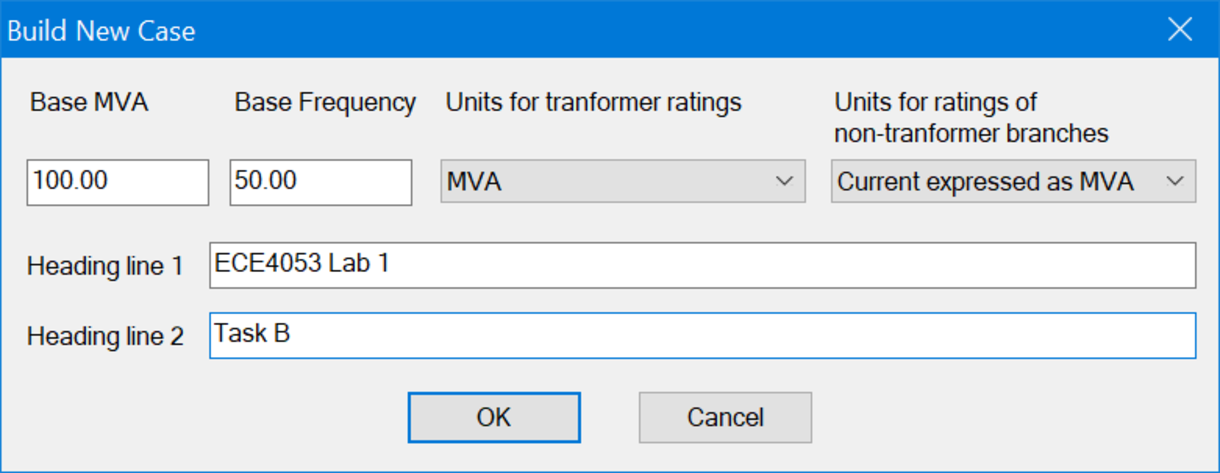
\includegraphics[scale=0.32]{fig8_newcase.pdf}
\caption{New case dialogue box}
\label{fig:8}
\end{figure}

Now the spreadsheet viewer should appear in the main area. In the ``Bus'' tab enter the first row from Table \ref{table:2}. Observe that while editing a row, the \mychar{pencil.png} appears on the left most column. When you are finished entering the data for a row, click the \mychar{star.png} icon on the last row to commit the changes.

In order to save the case, use the menu bar \textbf{\textcolor{gray}{File \textgreater \phantom{ }Save Untitled Case}}. You will be presented with a dialogue box as shown in Fig. \ref{fig:9}. Click on the \mychar{browse.png} icon and navigate to the \texttt{taskB} folder and give the saved case a sensible name.

\begin{figure}[h]
\centering
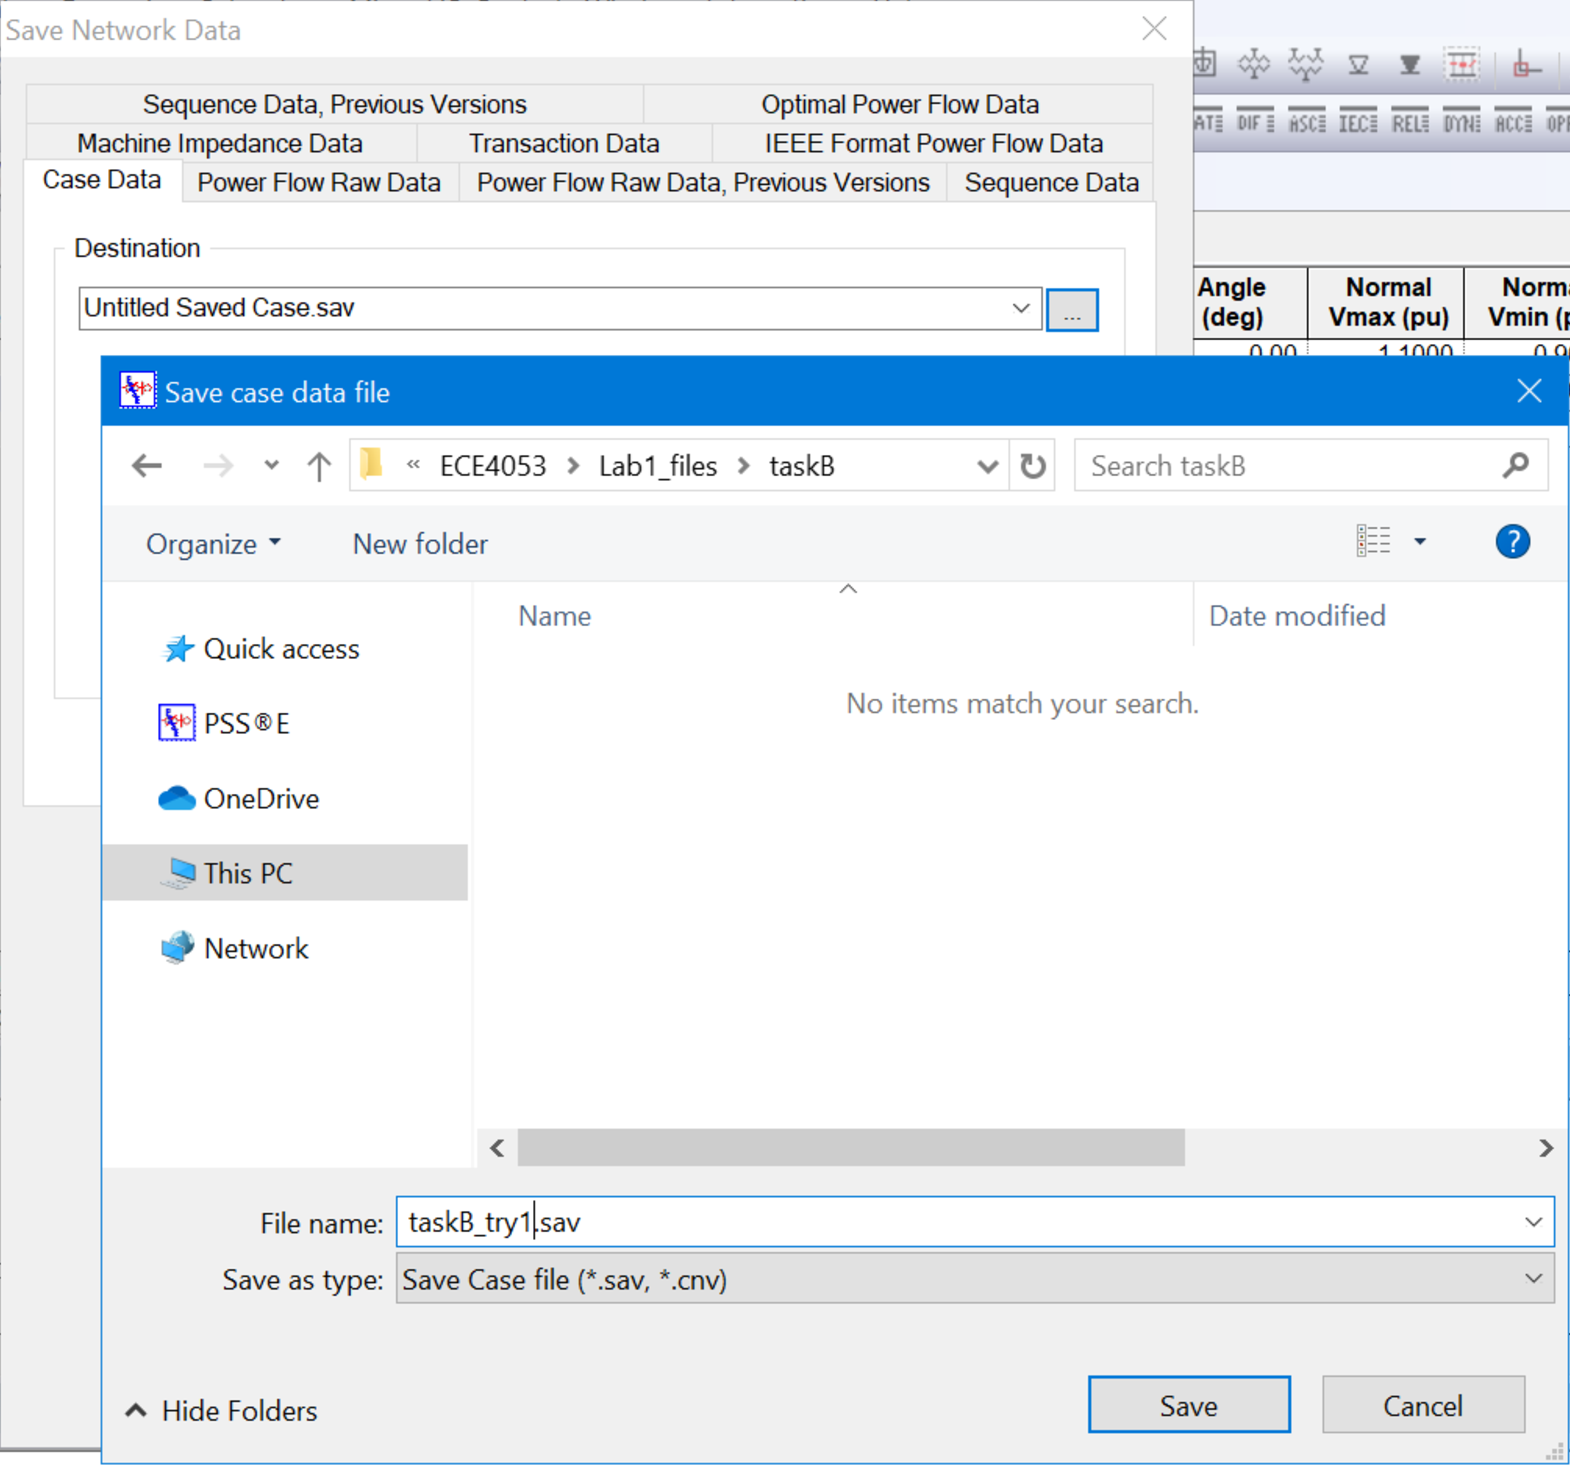
\includegraphics[scale=0.32]{fig9_save.pdf}
\caption{Saving the case data}
\label{fig:9}
\end{figure}

\subsubsection*{Activities}
\begin{enumerate}
\item[\textbf{6.3.1}] Can you match Tables 2, 3, 4, 5, 6, 7 and 8 to the corresponding spreadsheets in the spreadsheet viewer?
\item[\textbf{6.3.2}] Spend some time entering in the data into the spreadsheets. Do you have any suggestions to make this process quicker?
\end{enumerate}

\newpage
\subsection{Raw Data Files}
We can also prepare a saved case from raw data files. This is especially useful since some publically available models of power systems provide such raw files. The raw file format is a text file, so you can open it with a text editor. More information on how the data is formatted within the text file is provided \href{https://labs.ece.uw.edu/pstca/formats/pti.txt}{here}. For this lab, we have provided a raw file version of the power system defined in Section 6.2. Now we will see how we can load in this data.

Once again, it is a good idea to close and reopen PSS/E so that it starts fresh. Then from the menu bar choose: \textbf{\textcolor{gray}{File \textgreater \phantom{ }Open \textgreater \phantom{ }File}}. Navigate to the \texttt{taskB} folder and open the \texttt{taskB.raw} file.

It should open exactly like a saved case, with the data visible in the spreadsheets. Now we can follow the procedure outlined in Section 6.3 to save a .sav file.

\subsubsection*{Activities}
\begin{enumerate}
\item[\textbf{6.4.1}] As we found out in activity 6.3.1, the data entry process is prone to errors. Whenever you use someone else's model it is important to verify that the data is what you expect. By comparing the spreadsheeting with the tables in Section 6.2, correct any typos that occurred during the data entry process. (Hint: there are 5 typos.)
\end{enumerate}

\subsection{Creating a diagram}
In Section 5.5, we saw how useful a diagram is at graphically representing the tabular data. Now we will learn how to tell PSS/E to create a diagram for us. First, make sure you save your case data. Now using the menu bar: \textbf{\textcolor{gray}{File \textgreater \phantom{ }New \textgreater \phantom{ }Diagram}}. A blank diagram viewer will open in the main area. Use the menu bar again: \textbf{\textcolor{gray}{File \textgreater \phantom{ }Save As...}} and provide a sensible name. When saving a file, always ensure you are working in the appropriate directory.

An easy way to start a drawing is by clicking the ``Auto Draw'' icon \mychar{autodraw.png} located on the toolbar. Then left click anyway on the black canvas to open a dialogue box as shown in Fig. \ref{fig:10}. Click on the \textbf{\textcolor{gray}{Select...}} button, choose \texttt{BUS 100} and then click the \textbf{\textcolor{gray}{OK}} button on both dialogue boxes. A diagram should appear in the main area. Press ESC to exit the Auto Draw mode.

\begin{figure}[h]
\centering
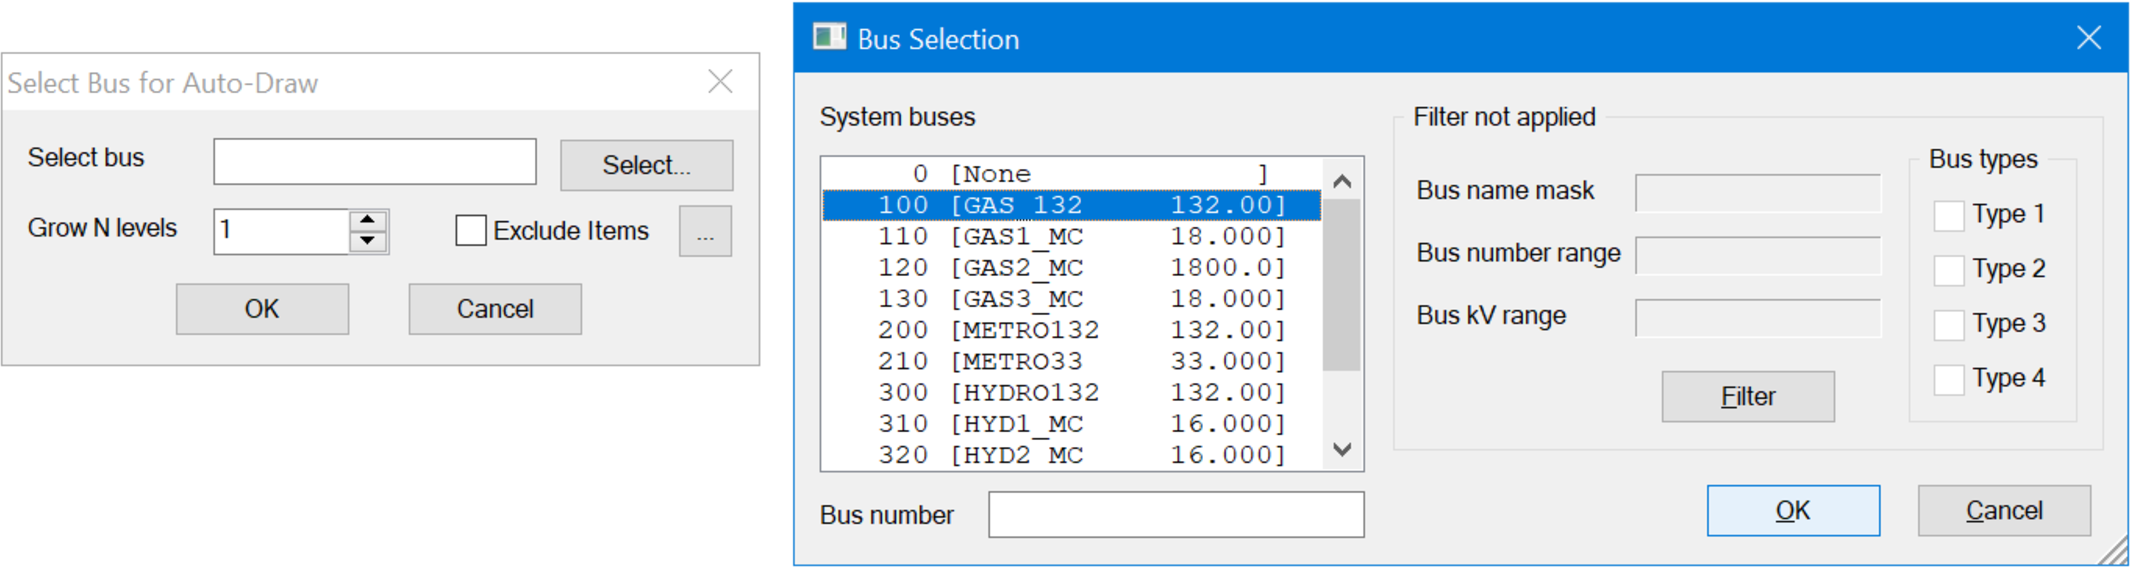
\includegraphics[scale=0.32]{fig10_autodraw.pdf}
\caption{Auto draw dialogue box}
\label{fig:10}
\end{figure}

\subsubsection*{Activities}
\begin{enumerate}
\item[\textbf{6.5.1}] How many buses are drawn? Can you explain why the full network was not drawn?
\item[\textbf{6.5.2}] Right click on bus 200 and click \textbf{\textcolor{gray}{Grow N levels...}}. What is the minimum number of levels you need to grow the network to capture the full power system?
\item[\textbf{6.5.3}] Now reorganise the diagram so that it resembles Fig. \ref{fig:7}. This can be done by dragging the buses to the appropriate locations and using the \mychar{rotate.png} icons on the toolbar if necessary.
\item[\textbf{6.5.4}] Save your work (both the diagram and case data). Then, on the diagram click on any bus and press the DELETE key. Now inspect the case data - are there any buses missing? Close PSS/E without saving changes.
\item[\textbf{6.5.5}] Reopen the case data and diagram. Now on the diagram viewer, use the menu bar to toggle  \textbf{\textcolor{gray}{Diagram \textgreater \phantom{ }Bind Changes to Network Data}}. Now delete a bus on the diagram again. What happened to the case data now?



\end{enumerate}


\newpage
\section{Conclusion}
Congratulations on finishing the first PSS/E! Next week we will build on this knowledge and learn how to perform load flow analysis with PSS/E.

One of the most important aspect of learning a new software is knowing where to find help. Below are some suggestions:
\begin{enumerate}
\item Google search: often your question might have been addressed in an online forum.
\item PSS/E built in help: pressing F1 on your keyboard brings up the PSS/E help that is indexed by keywords.
\item PSS/E manual: this is available on Moodle and should contain the answer to your question. Being able to navigate through technical manuals is an invaluable skill for industry.
\item Moodle discussion forum: this is a great place to ask and answer questions.
\item Your lab peers and demonstrators: feel free to ask any question. Being able to ask for help if you are stuck is another crucial skill.
\end{enumerate}
\end{document}